%!TEX root = ../thesis.tex
%*******************************************************************************
%****************************** Second Chapter *********************************
%*******************************************************************************

\chapter{Experimental} % 1200 words as of sept 22

\ifpdf
    \graphicspath{{Chapter2/Figs/Raster/}{Chapter2/Figs/PDF/}{Chapter2/Figs/}}
\else
    \graphicspath{{Chapter2/Figs/Vector/}{Chapter2/Figs/}}
\fi


\section[Preparation of samples]{Preparation of pigment samples} 
\label{section2.1}

Reference samples were acquired from Dr. Spike Bucklow from the Hamilton Kerr Institute collection and Dr. Andrea Kirkham from her sample library. All reference samples were loose powder and are described qualitatively in Table \ref{table:ref_sample}. The sample descriptions provided formed the basis for interpretation of results (and some terminology such as "bice" is used to describe both natural and synthetic pigments---this ambiguity is discussed when analysing results). Samples are pictured in storage in \textit{Figures \ref{fig:sample_bags}} and \textit{\ref{fig:sample_vials}}, and pressed on slides for confocal Raman analysis in \textit{Figure \ref{fig:sample_slides}}.

Prior to Raman analysis, small quantities of each pigment were pressed onto double-sided sellotape and smoothed using a metal spatula. Prior to SEM-EDS analysis, small quantities of each pigment were pressed onto high purity conductive double-sided adhesive carbon tabs to minimise surface charging.

\begin{table}[H]
\caption{Reference sample descriptions}
\centering
\label{table:ref_sample}
\begin{tabular}{c c}
\toprule
Reference sample & Qualitative physical description \\
\midrule
HKI natural azurite & Natural azurite, medium sandy blue \\
HKI cross section & Natural and artifical azurite \\
KE 1a, KE 1b & Green bice, light pale teal green \\
KE 2 & Green verditer, CuCO\textsubscript{3} $\cdot$ Cu(OH)\textsubscript{2}, bright teal green \\
KE 3 & Light verditer bice, medium dark blue \\
KE 4 & Blue bice, medium grey blue \\
KE 5 & Blue verditer, 2CuCO\textsubscript{3} $\cdot$ Cu(OH)\textsubscript{2}, dark blue \\
Fitz 1 & Blue verditer, Fitzpatrick 10180, dark blue \\
Az 1 & Azurite, medium light blue \\
Az 2 & Azurite, dark deep blue \\
Az Op & Azurite, medium blue \\
Az Mag & Azurite, medium teal blue \\
Ma 1 & Malachite, medium light green \\
\bottomrule
\end{tabular}
\end{table}

\begin{figure}[H]
\centering
  \includegraphics[width=0.75\linewidth]{sample_bags}
\caption[Samples KE 1-5 and Fitz 1.]{Samples KE 1-5 and Fitz 1 shown in storage bags.}
\label{fig:sample_bags}
\end{figure}

\begin{figure}[H]
\centering
  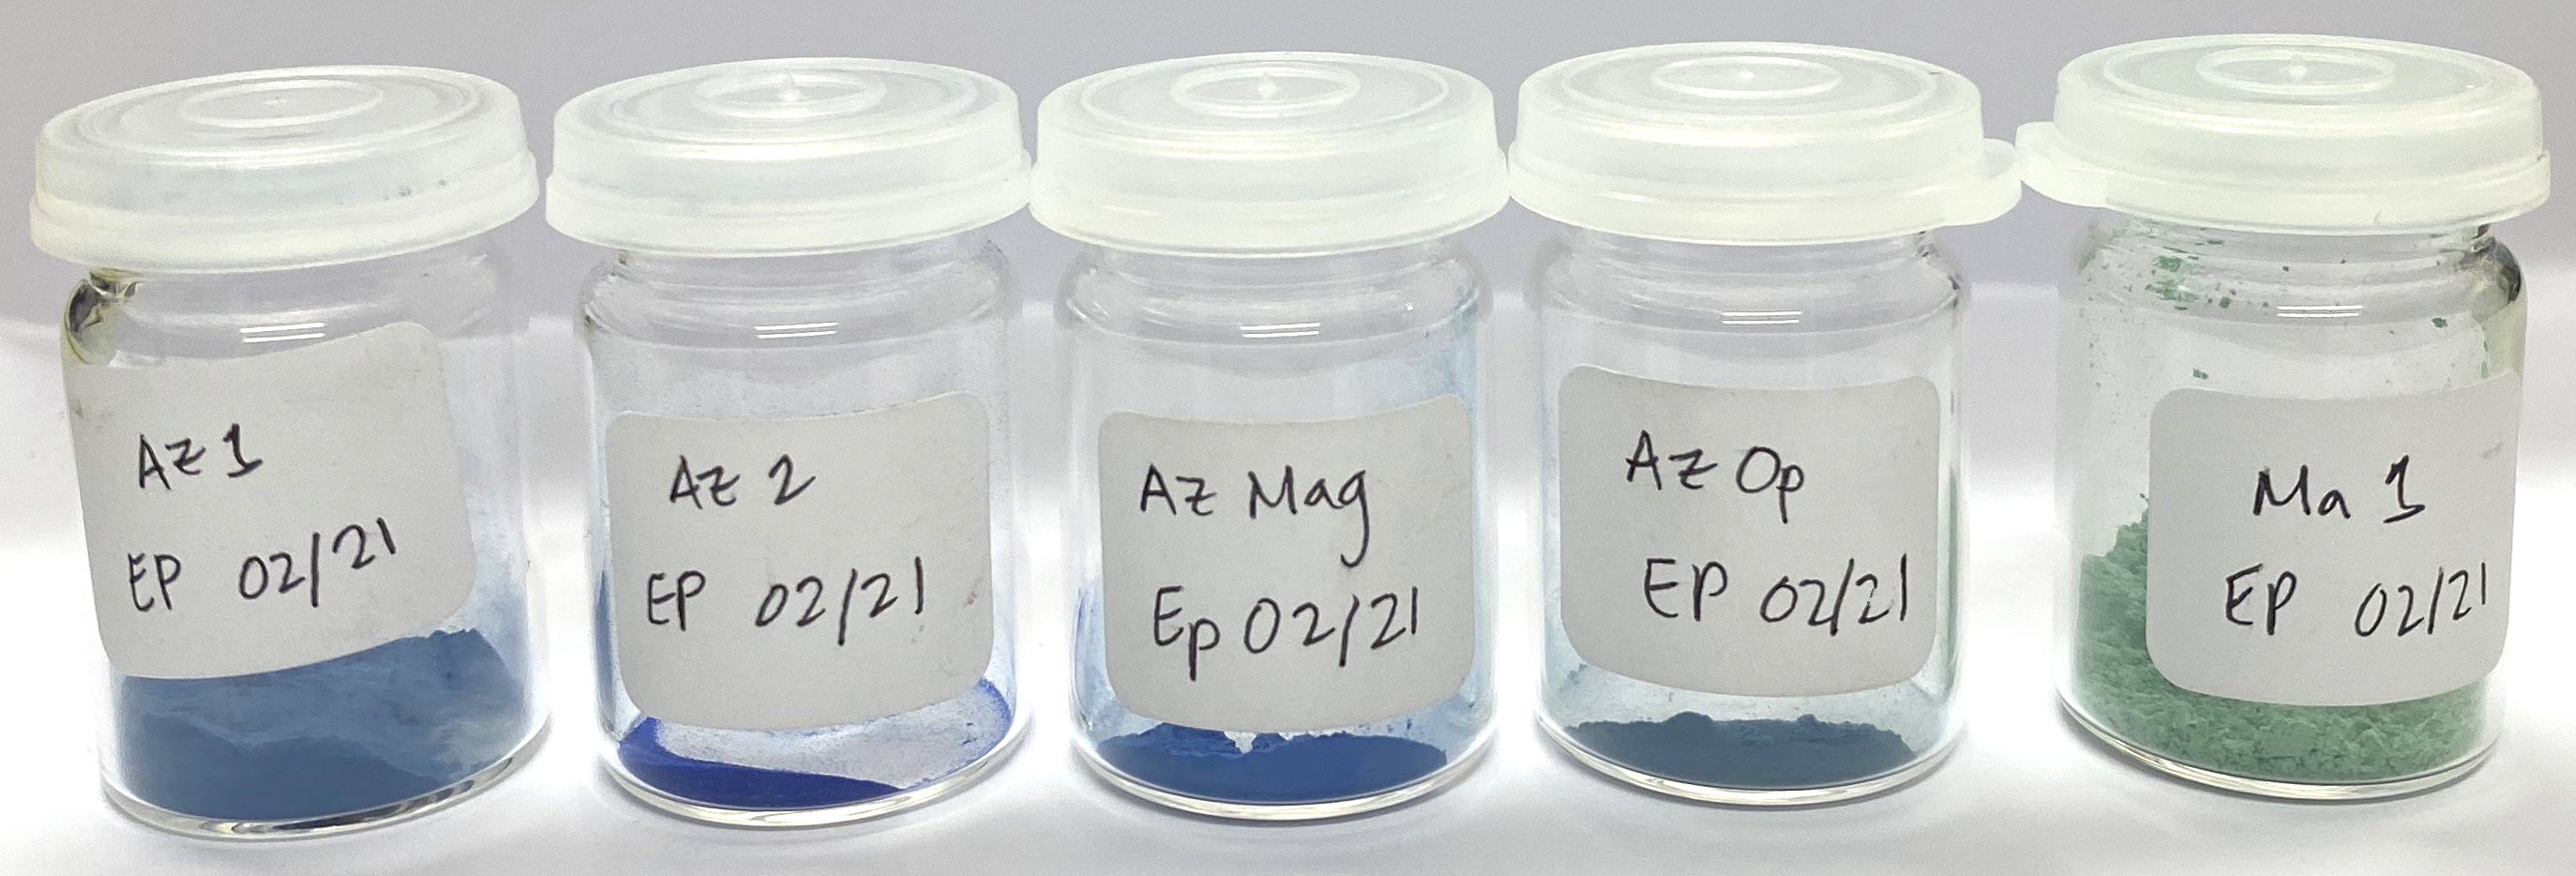
\includegraphics[width=0.75\linewidth]{sample_vials}
\caption[Samples Az 1, Az 2, Az Op, Az Mag, and Ma 1.]{Samples Az 1, Az 2, Az Op, Az Mag, and Ma 1, shown in small sample vials.}
\label{fig:sample_vials}
\end{figure}

\begin{figure}[H]
\centering
  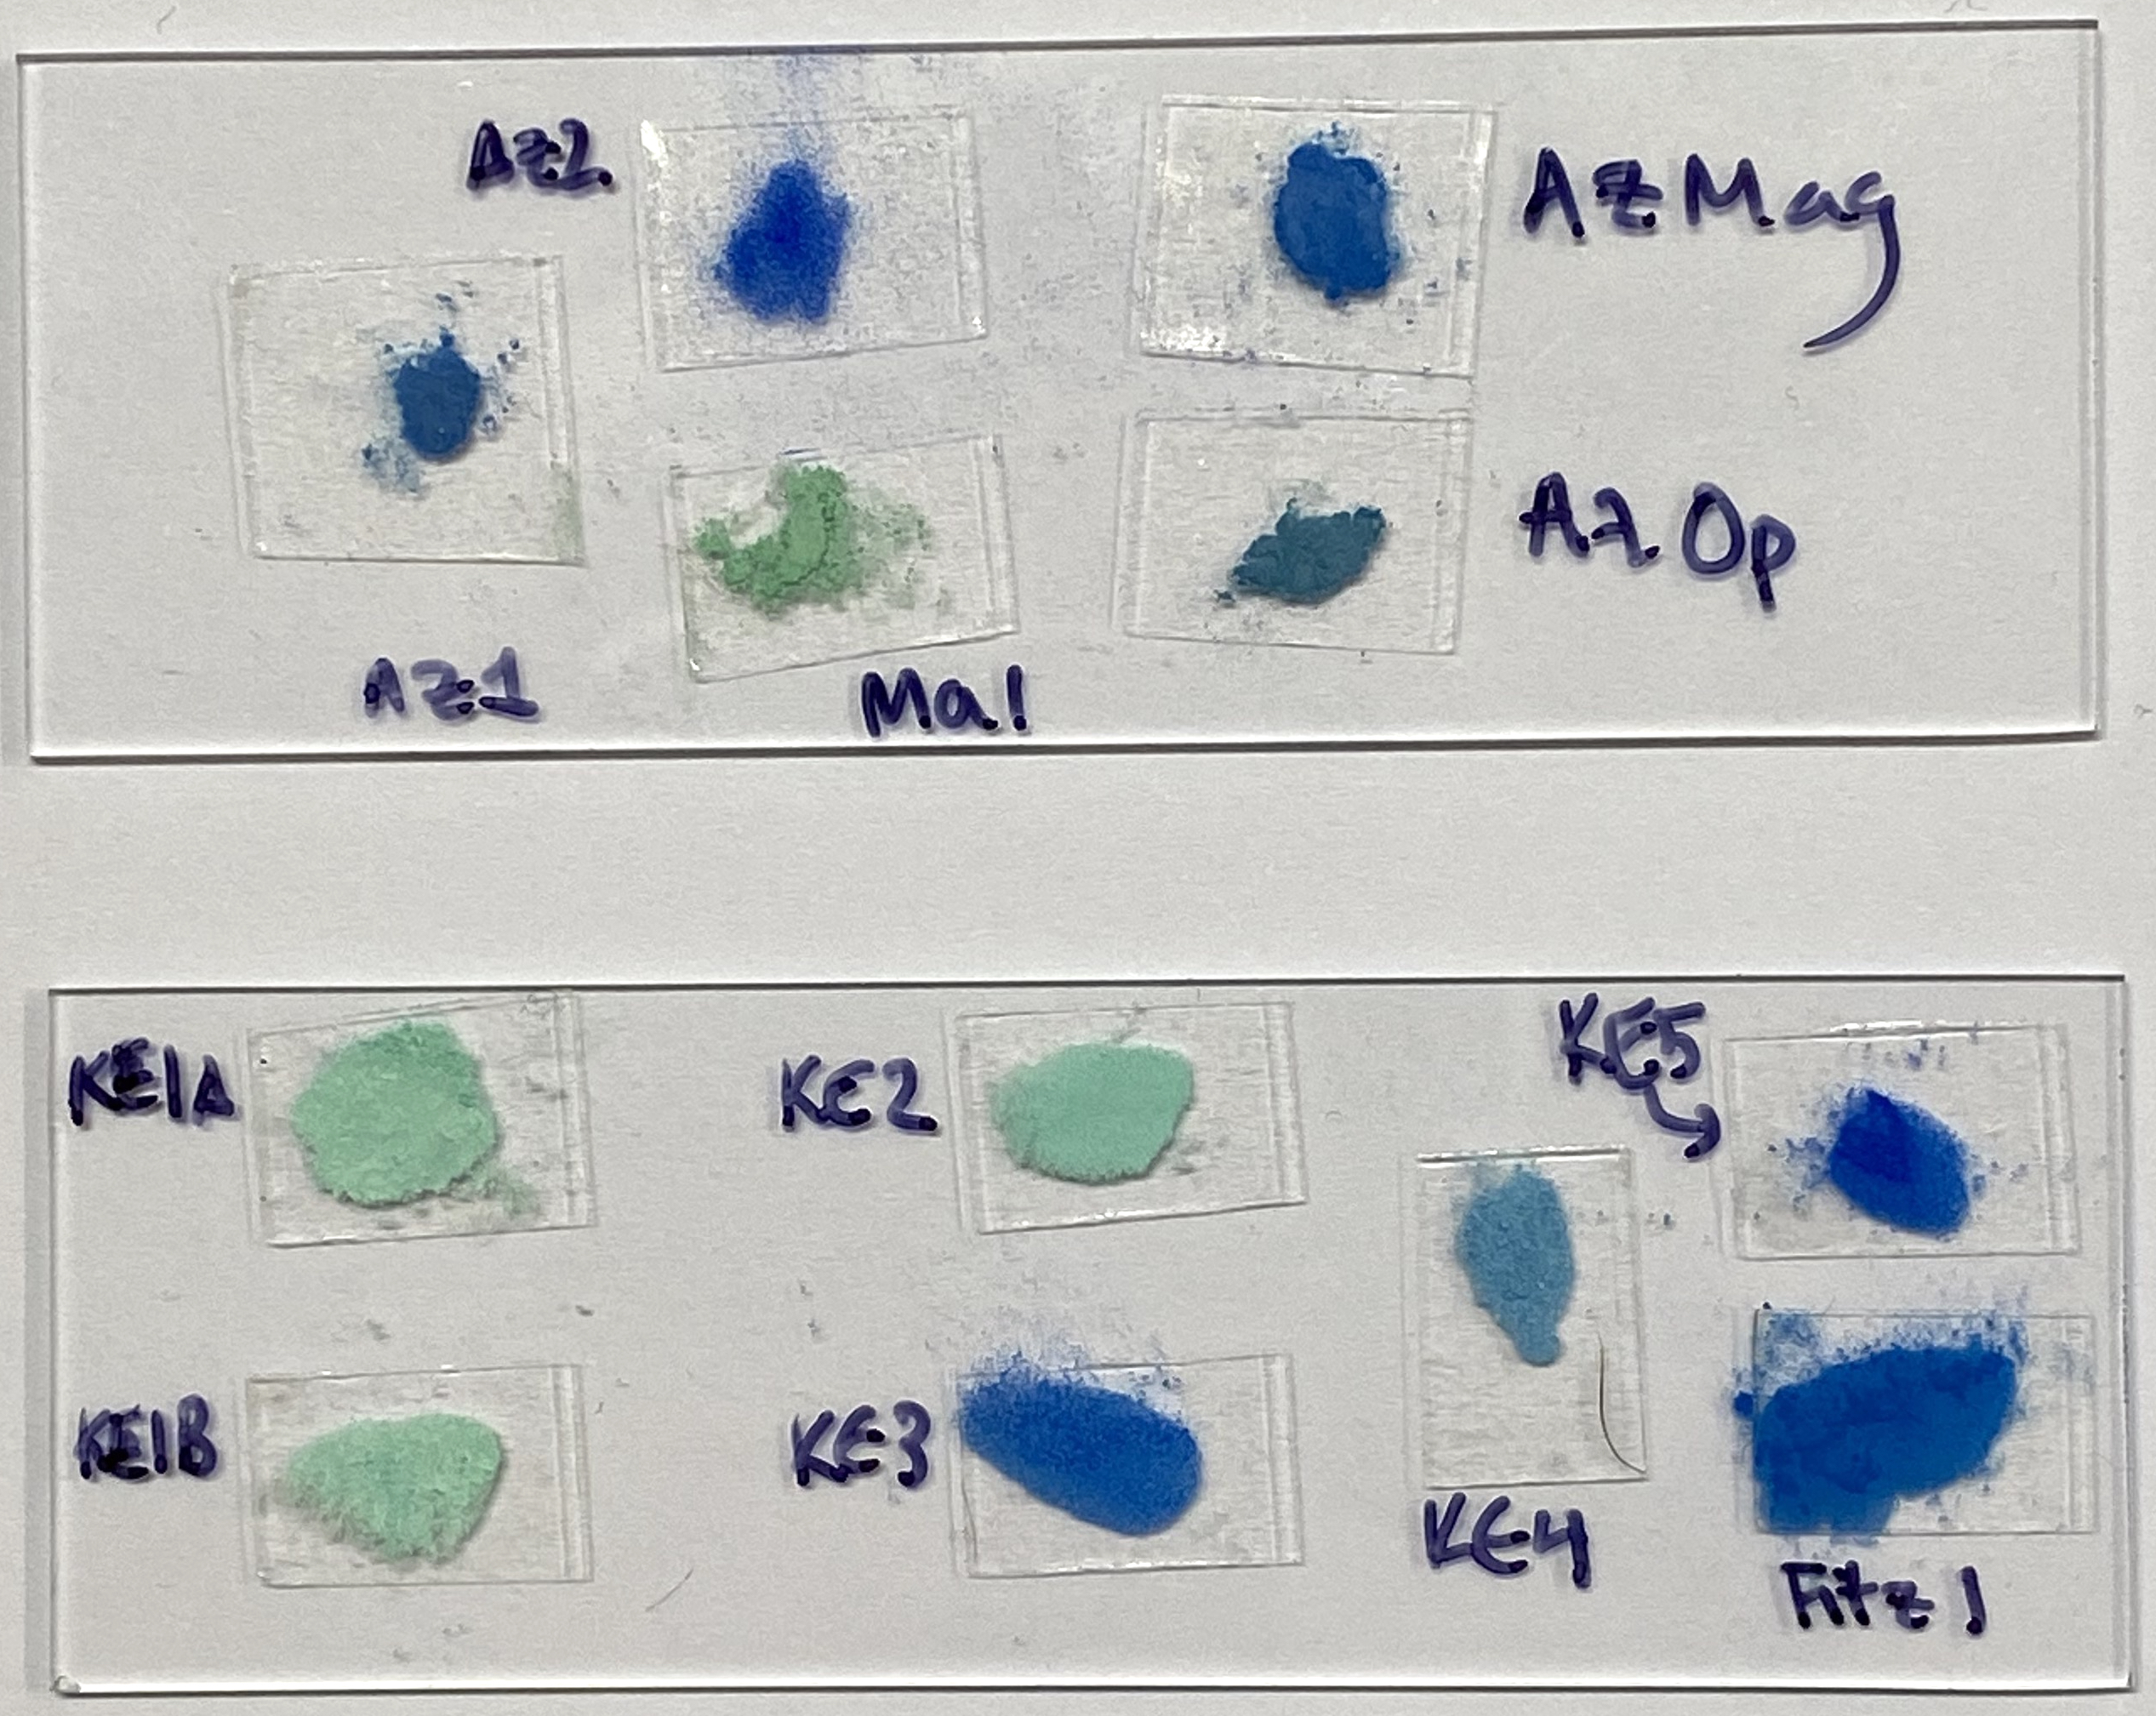
\includegraphics[width=0.75\linewidth]{sample_slides}
\caption[All reference samples shown pressed on double-sided tape and prepared for Raman analysis.]{All reference samples shown pressed on double-sided tape and prepared for Raman analysis.}
\label{fig:sample_slides}
\end{figure}

Pigment samples were also embedded in resin and polished to create a flat, uniform surface for Raman mapping and AFM analysis. A small quantity of pigment was placed in a coin shaped mold and a clear polyester resin (Tiranti clear casting resin) was poured over the pigment. The resin was allowed to set for 48 hours before being removed from the mold. Samples were filed to approximately 5 mm in height and the pigment containing surface was polished using three sequential grit sizes of silicon carbide paper (English Abrasives) and polishing cloth (Buehler), using a fine grade cerium oxide polishing powder (Beckman-RIIC) in ethanol. Finally, polished samples were cleaned with ethanol to remove extra polish and debris prior to analysis.

\section[Analysis of pigment particles by Raman spectroscopy]{Analysis of pigment particles by Raman spectroscopy}
\label{section2.2}

Collection of Raman spectra of pigment samples was done using a Horiba LabRAM HR Evolution confocal Raman spectrometer with a 50x microscope objective (Olympus LMPLFLN), a 600 grooves/mm grating, and a CCD array (1024x1024 pixels). The pinhole size was 100 $\mu$m. An laser with excitation wavelength of 532 nm (diode-pumped solid-state, Laser Quantum) was initially selected based on optimal signal to noise ratio with lack of sample damage. We expect that the samples under consideration in this study, azurite and malachite, will show strong signals at 532 nm based on previous work on these materials.~\autocite{Bicchieri} References were also collected at 473 nm (Cobolt, 1800 grooves/mm grating, 150 $\mu$m pinhole), which showed superior results for blue samples due to high reflection but did not perform as well on green samples. Two other excitation wavelengths, 633 nm and 785 nm, were also tested and found to give inferior results at longer acquisition times and/or higher laser powers at the sample surface, as shown in \textit{Figure \ref{fig:Az1_wavelength_comparison}}. Spectra were collected in the confocal mode focusing on specific pigment grains.

Resin-embedded cross section samples from \textit{Battle of Spurs} were studied using the same parameters and procedures.

\begin{figure}[H]
\centering
  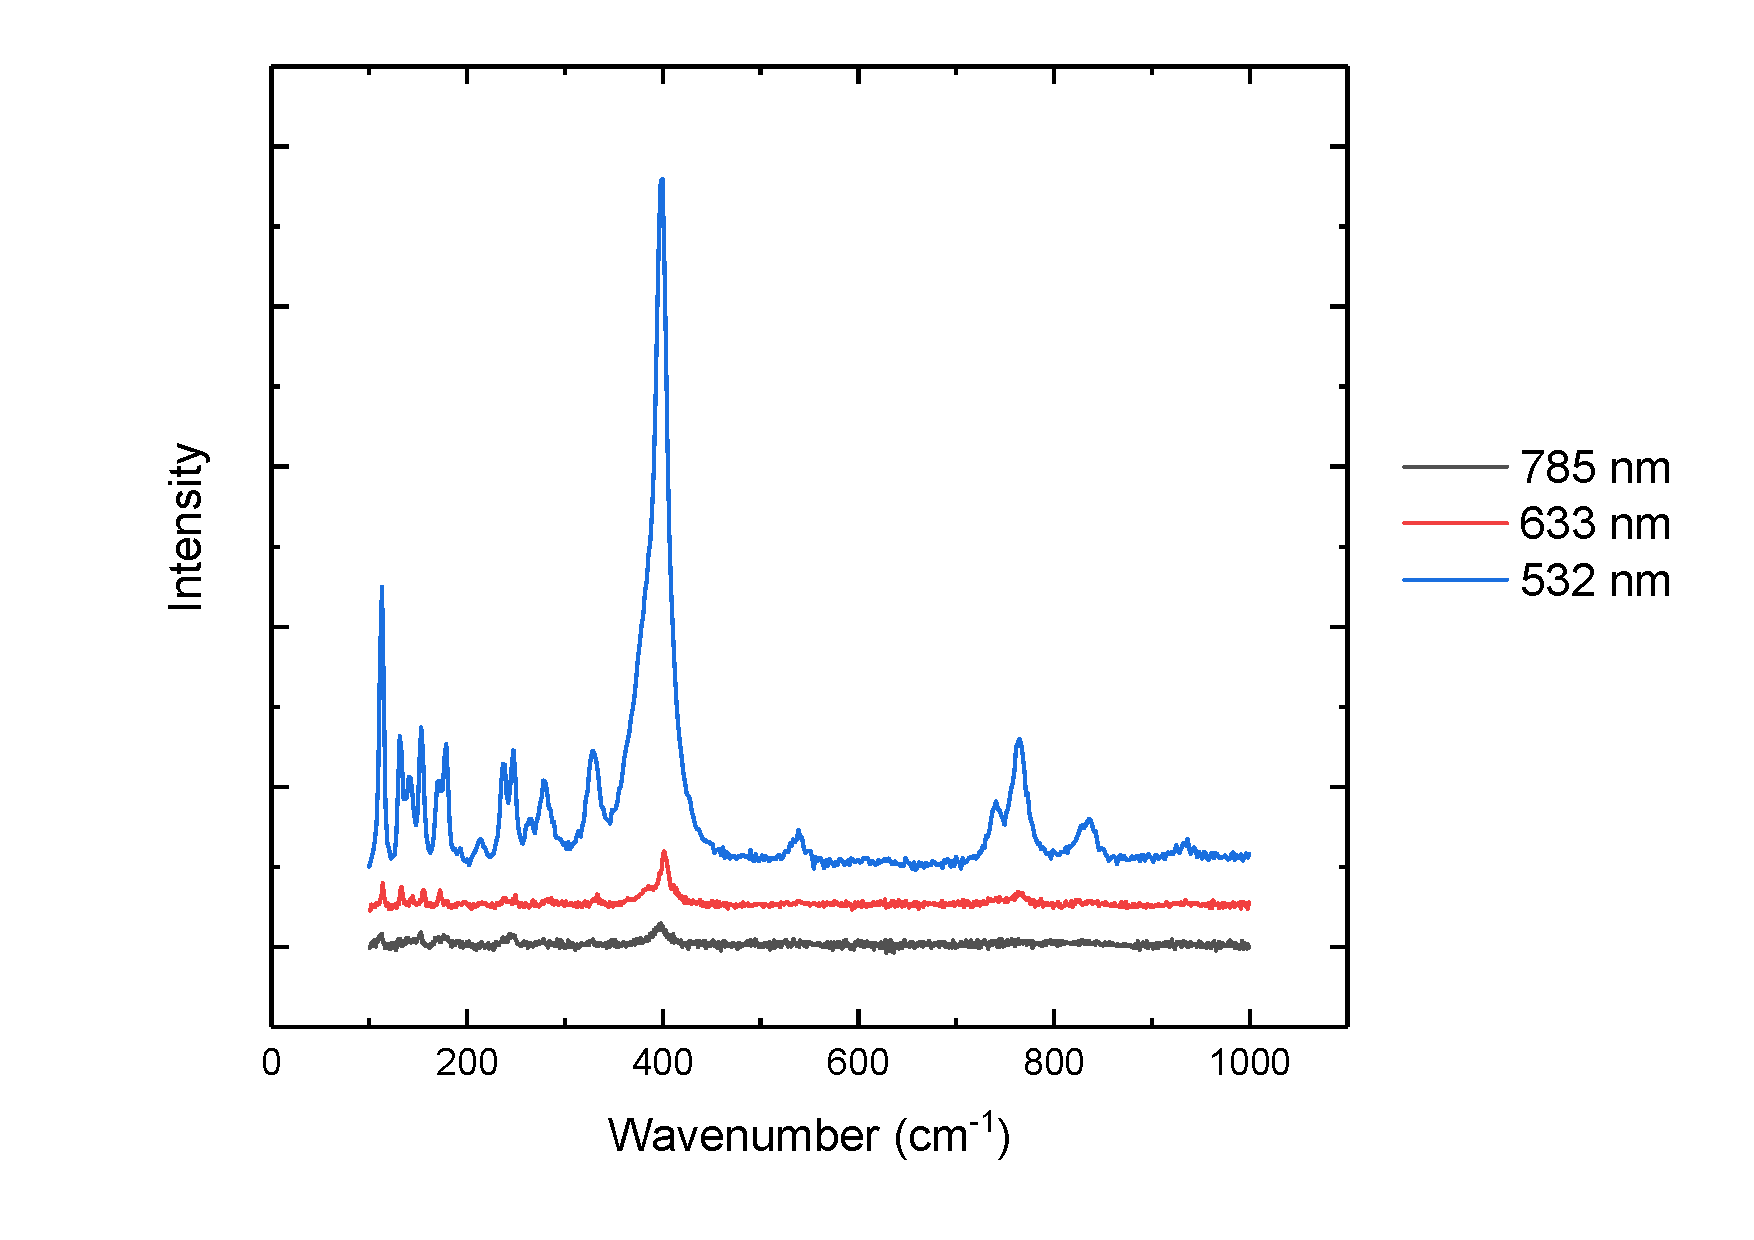
\includegraphics[width=0.75\linewidth]{Az1_wavelength_comparison}
\caption[Comparison of spectra collected at 473, 532, 633, and 785 nm excitation wavelengths from sample Az 1.]{Comparison of spectra collected at 473 (green), 532 (blue), 633 (red), and 785 nm (black) excitation wavelengths from sample Az 1.}
\label{fig:Az1_wavelength_comparison}
\end{figure}

Optimal collection parameters were determined to maximise the signal to noise ratio of spectra while avoiding sample damage and minimising collection times (\textit{Figure \ref{fig:Az1_laserpower_comp_532}}). The damage threshold of pigment grains was observed to depend on the sample identity and the size of the grain sampled. This has been observed in previous studies and is expected.~\autocite{Cardell,Mattei} Damage to azurite (blue bice, blue verditer) samples was observed to occur at 50\% power or 4 mW with an acquisition time of 10 s and 10 accumulations. Malachite (green verditer) has a lower damage threshold, occurring at at 25\% power or 2 mW with an acquisition time of 10 s and 10 accumulations. 10\% power or 1 mW with an acquisition time of 10 s and 10 accumulations did not cause observable damage to any reference sample. For the sake of consistency, this lower surface power and acquisition time was selected for all samples as it gave a satisfactory signal quality. 

\begin{figure}[H]
\centering
  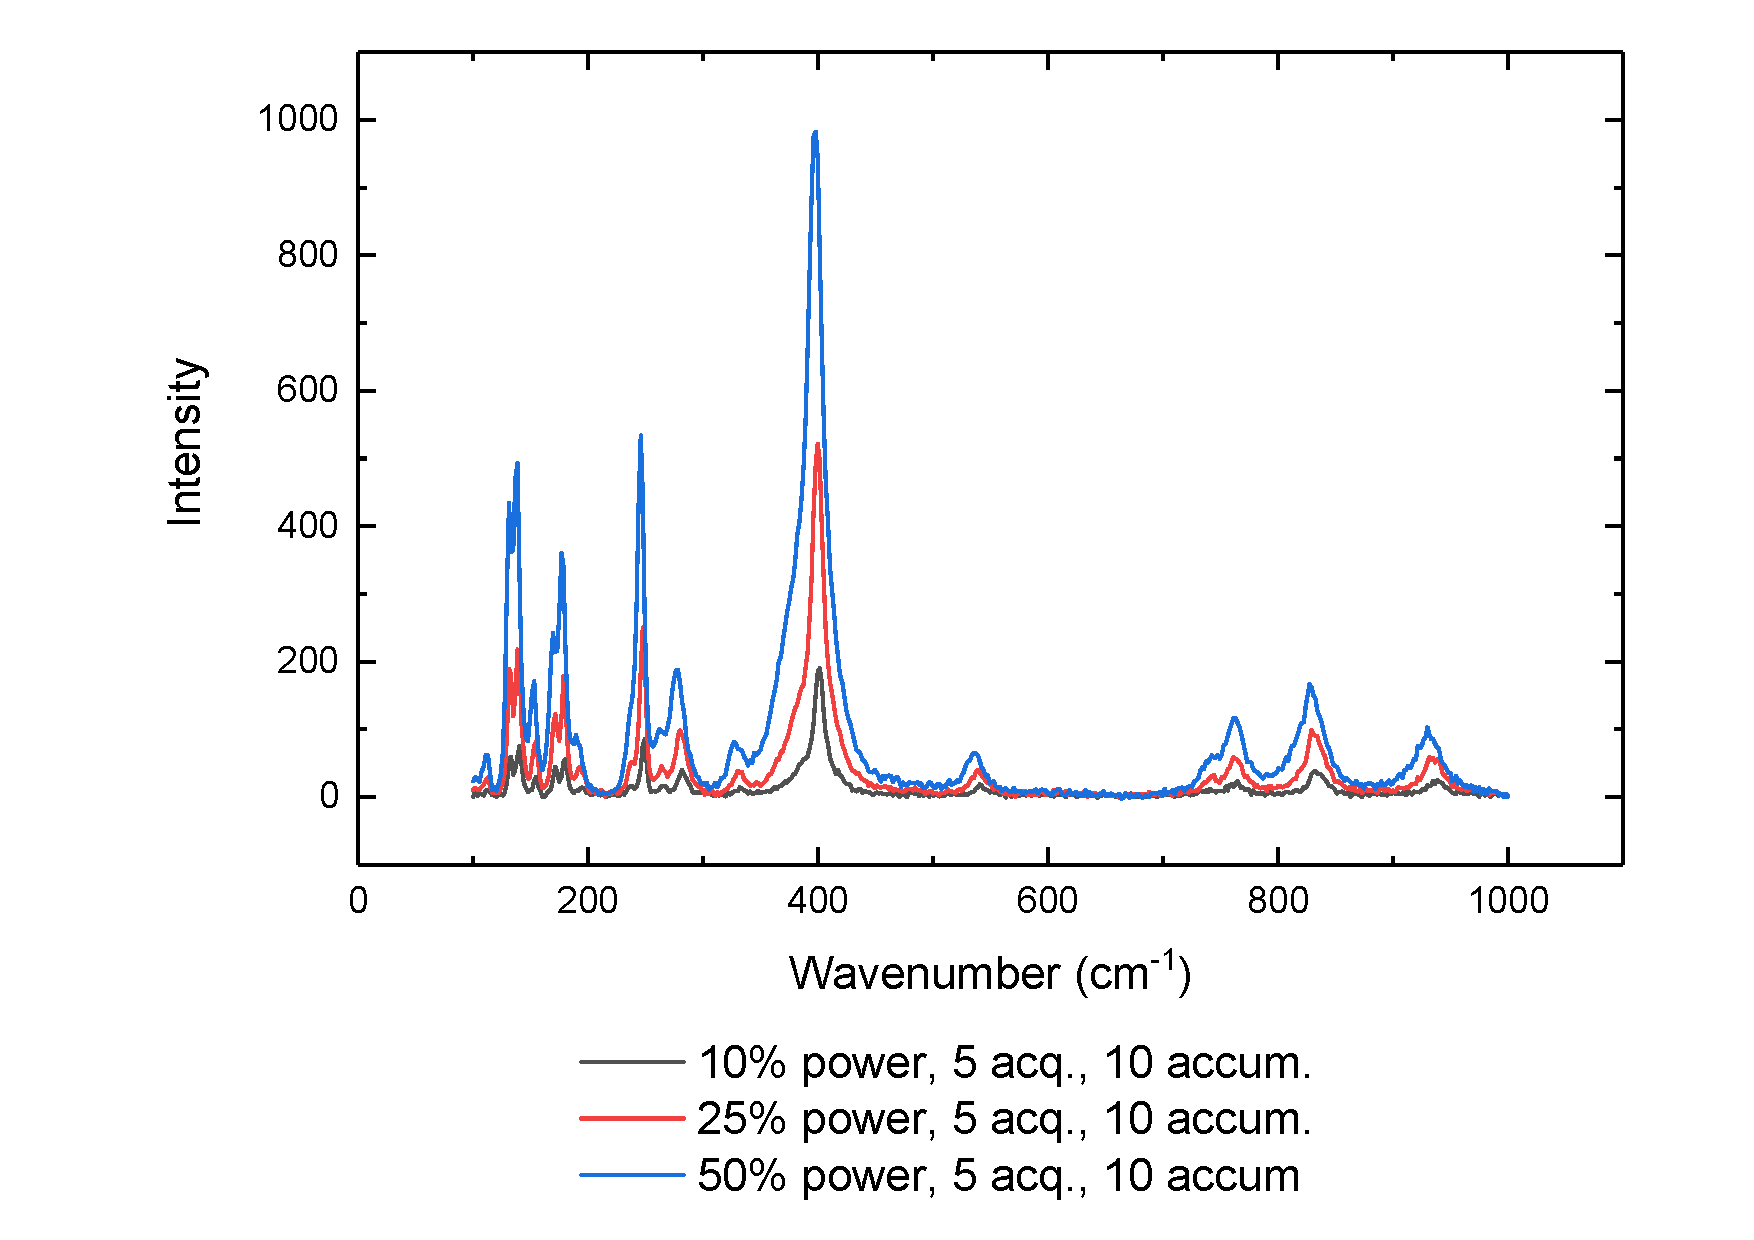
\includegraphics[width=0.75\linewidth]{Az1_laserpower_comp_532}
\caption[Comparison of spectra collected using 532 nm excitation wavelength at 10\%, 25\%, and 50\% power.]{Comparison of spectra collected using 532 nm excitation wavelength at 10\% (black), 25\% (red), and 50\% (blue) power (5 acquisitions, 10 accumulations).}
\label{fig:Az1_laserpower_comp_532}
\end{figure}

Raman spectra were processed using OriginPro 2017 software. All spectra were fit to a spline baseline. 

\section[Analysis of pigment particles by SEM-EDS]{Analysis of pigment particles by SEM-EDS}
\label{section2.3}

Pigment particle shape, size, and regularity, as well as elemental composition, were characterized using scanning electron microscopy (SEM) coupled to energy dispersive X-ray spectroscopy (EDS). Samples were prepared as described in section \ref{section2.1}. Micrographs of pigments were collected at several magnifications rangeing from 250x to 2500x using a JEOL JSM-5510LV scanning electron microscope, imaged using the secondary electron detector. The working distance between the sample and the beam source was 20 mm. The accelerating voltage was 10 keV, which caused minimal charging on the surface of the sample, unless otherwise noted. ED spectra were collected at the same time as SEM imaging using an Oxford instruments INCA EDX detector and software. The accelerating voltage was 10 keV unless otherwise noted, which limited detection of heavier elements but minimized surface charging. Elemental mapping using EDS was also carried out to detect variation between pigment grains within the same sample and identify local differences.

Resin embedded cross section samples were studied using the same procedure outlined above. Prior to SEM-EDS analysis, cross sections were coated with a 25 nm layer of amorphous carbon and resin around the sample area was covered with copper metal. This minimised surface charging in the instrument.

\section[Analysis of pigment particles by AFM-IR]{Analysis of pigment particles by AFM-IR}
\label{section2.4}

Resin-embedded powder samples and cross sections were studied using an Anasys NanoIR2 instrument in both contact and tapping modes. Height, deflection, and phase maps were collected in tapping mode using a HQ:NSC15 Al probe (Mikro Masch, 265-410 kHz resonant frequency, 20-80 N/m force constant). Map areas ranged from 80 x 80 $\mu$m to 2 x 2 $\mu$m with resolution of 250 x 250 pixels and a scan rate of 0.1 Hz. 

Infrared maps and spectra were collected in contact mode using an ATEC-CONTAu-10 gold-coated silicon probe (7-25 kHz resonant frequency, 0.02-0.75 N/m spring constant, Nanosensors). Four quantum cascade lasers (Daylight Solutions) spanning a total range of 1125-2298 cm\textsuperscript{-1} were used for infrared spectra collection. The laser power used was 10.98\%. Infrared mapping was carried out at several frequencies discussed in analysis.

%The duty cycle was 3\%. 

\section[Bulk sample analysis by ATR FT-IR]{Bulk sample analysis by attenuated total reflectance infrared spectroscopy}
\label{section2.5}

Attenuated total reflectance (ATR) infrared spectra were collected using a Bruker Vertex 70 FT-IR spectrometer equipped with a gold ATR accessory and a liquid nitrogen cooled MCT mid-IR detector. OPUS software was used for collection. A background spectrum was collected before each sample spectrum using the clean ATR crystal (200 scans). Each sample spectrum was collected from solid powder/resin with 200 scans co-averaged and a resolution of 4 cm\textsuperscript{-1}. Spectra were processed using OriginPro 2017 software by fitting a spline baseline to transmission spectra and subtracting. Data was converted from transmittance to absorbance as needed for comparison to AFM-IR spectra using the formula A = 2 - log(\%T).


